	\newcommand{\class}[1]{\paragraph{Klasse #1:}\ \\ }
	\newcommand{\method}[1]{\textcolor{blue}{#1}}
	\newcommand{\kursiv}[1]{{\it #1}}
	\newcommand{\override}{{\it @Override}\ \\}
	
	\chapter{Klassenbeschreibung und Klassendiagramm}
	In diesem Kapitel werden alle Klassen der Anwendung \textbf{ofCourse} aufgeführt.
	Um eine bessere Übersicht und Strukturierung zu erhalten wird das ganze Projekt in Packages aufgeteilt.

	\section{Package Action}
		\begin{tiny}
			TF\\
		\end{tiny}\\
	Dieses Package stellt die Businesslogik des Systems \textbf{ofCourse} dar.
	\subsection{Klasse AuthenticateUser}
	\kursiv{ManagedBean, RequestScoped}\\
	Die Klasse ist für die Authentifizierung eines Benutzers im System zuständig.
	\begin{itemize}
		\item \method{public boolean login()}
		\item \method{public User getLoginUser()}
		\item \method{public void setLoginUser(User userToLogIn)}
		\item \method{public SessionUser getSessionUser()}
		\item \method{public void setSessionUser(SessionUser userSession)}
	\end{itemize}
	
	\subsection{Klasse RegisterUser}
	\kursiv{ManagedBean, RequestScoped}\\
	Die Klasse ist für die Registrierung eines Benutzers im System zuständig.
	\begin{itemize}
		\item \method{public boolean registerUser()}
		\item \method{public User getUsertoRegistrate()}
		\item \method{public void setUserToRegistrate(User userToRegistrate)}
		\item \method{public Address getAddress()}
		\item \method{public void setAddress(Address addressToSet)}
		\item \method{public SessionUser getSessionUser()}
		\item \method{public void setSessionUser(SessionUser userSession)}
	\end{itemize}
	
	\subsection{Klasse LostPassword}
	\kursiv{ManagedBean, RequestScoped}\\
	Die Klasse ist für die 'Passwort  vergessen' - Funktion zuständig, d.h. sie ersetzt das alte Passwort eines Benutzers durch ein zufällig generiertes und sendet es an die eingegebene E-Mailadresse.
	\begin{itemize}
		\item \method{public boolean resetPassword()}
		\item \method{public String getEmailAddressToResetPassword()}
		\item \method{public void setEmailAddressToResetPassword(String emailToResetPassword)}
		\item \method{public User getUser()}
		\item \method{public void setUser(User user)}
	\end{itemize}
	
	\subsection{Klasse SearchUser}
	\kursiv{ManagedBean, ViewScoped}\\
	Diese Klasse stellt den Mechanismus zum Suchen von Benutzern zur Verfügung.
	\begin{itemize}
		\item \method{public ArrayList<User> getSearchResult()}
		\item \method{public void setSearchResult(ArrayList<User> searchResult)}
		\item \method{public void search(String searchParam, String searchTerm)}
		\item \method{public String getSearchParam()}
		\item \method{public void setSearchParam(String searchParam)}
		\item \method{public String getSearchTerm()}
		\item \method{public void setSearchTerm(String searchTerm)}
		\item \method{public void sortBySpecificColumn()}
		\item \method{public int getActualPageNumber()}
		\item \method{public void goToSpecificPage()}
		\item \method{public Pagination getPagination()}
		\item \method{public void setPagination(Pagination pagination)}
		\item \method{public SessionUser getSessionUser()}
		\item \method{public void setSessionUser(SessionUser userSession)}
	\end{itemize}
	
	\subsection{Klasse SearchCourse}
	\kursiv{ManagedBean, ViewScoped}\\
	Diese Klasse stellt den Mechanismus zum Suchen von Kursen zur Verfügung. Außerdem wird darin die Einschränkung des angezeigten Kursangebots realisiert.
	\begin{itemize}
		\item \method{public void searchForFreeCourses()}
		\item \method{public void displayCoursesInSpecificPeriod()}
		\item \method{public String getDisplayPeriod()}
		\item \method{public void setDisplayPeriod(String displayPeriod)}
		\item \method{public ArrayList<Course> getSearchResult()}
		\item \method{public void setSearchResult(ArrayList<Course> searchResult)}
		\item \method{public void search(String searchParam, String searchTerm)}
		\item \method{public String getSearchParam()}
		\item \method{public void setSearchParam(String searchParam)}
		\item \method{public String getSearchTerm()}
		\item \method{public void setSearchTerm(String searchTerm)}
		\item \method{public void sortBySpecificColumn()}
		\item \method{public int getActualPageNumber()}
		\item \method{public void goToSpecificPage()}
		\item \method{public Pagination getPagination()}
		\item \method{public void setPagination(Pagination pagination)}
		\item \method{public SessionUser getSessionUser()}
		\item \method{public void setSessionUser(SessionUser userSession)}
	\end{itemize}
	
	\subsection{Klasse UserProfil}
	\kursiv{ManagedBean, ViewScoped}\\
	Diese Klasse ist zuständig für die Anzeige und das Bearbeiten der Benutzerdaten. Des Weiteren realisiert sie die Darstellung der Liste aller vom Benutzer geleiteten Kurse.
	\begin{itemize}
		\item \method{public void editUserdata()}
		\item \method{public void saveUserdata()}
		\item \method{public boolean uploadProfilPic()}
		\item \method{public void setUserInactive()}
		\item \method{public void depositMoneyPerCreditcard()}
		\item \method{public User getUser()}
		\item \method{public void setUser(User userToSet)}
		\item \method{public Address getAddress()}
		\item \method{public void setAddress(Address addressToSet)}
		\item \method{public ArrayList<Course> getManagedCourses()}
		\item \method{public void setManagedCourses(ArrayList<Course> managedCourses)}
		\item \method{public int getActualPageNumber()}
		\item \method{public void goToSpecificPage()}
		\item \method{public Pagination getPagination()}
		\item \method{public void setPagination(Pagination pagination)}
		\item \method{public SessionUser getSessionUser()}
		\item \method{public void setSessionUser(SessionUser userSession)}
	\end{itemize}
	
	\subsection{Klasse CourseDetail}
	\kursiv{ManagedBean, ViewScoped}\\
	Die Klasse ist zuständig für die Anzeige der Kursdetails und das Bearbeiten von Kursen.
	\begin{itemize}
		\item \method{public void editCourse()}
		\item \method{public boolean saveCourse()}
		\item \method{public Course getCourse()}
		\item \method{public void setCourse(Course course)}
		\item \method{public boolean registeredForCourseNews()}
		\item \method{public String signUpForCourse() throws CourseRegistrationException}
		\item \method{public String signOffFromCourse() throws CourseRegistrationException}
		\item \method{public void selectAllCourseUnits()}
		\item \method{public String signUpForCourseUnits() throws CourseRegistrationException}
		\item \method{public String signOffFromCourseUnits() throws CourseRegistrationException}
		\item \method{public ArrayList<CourseUnit> getSelectedCourseUnits()}
		\item \method{public void setSelectedCourseUnits(ArrayList<CourseUnit> selectedCourseUnits)}
		\item \method{public ArrayList<User> getLeadersOfCourse()}
		\item \method{public void setLeadersOfCourse(ArrayList<User> leaders)}
		\item \method{public ArrayList<CourseUnit> getCourseUnitsOfCourse()}
		\item \method{public void setCourseUnitsOfCourse(ArrayList<CourseUnit> courseUnits)}
		\item \method{public String loadParticipientsPage()}
		\item \method{public String loadCreateCourseUnitPage()}
		\item \method{public String loadEditCourseUnitPage()}
		\item \method{public int getActualPageNumber()}
		\item \method{public void goToSpecificPage()}
		\item \method{public Pagination getPagination()}
		\item \method{public void setPagination(Pagination pagination)}
		\item \method{public SessionUser getSessionUser()}
		\item \method{public void setSessionUser(SessionUser userSession)}
	\end{itemize}
	
	\subsection{Klasse CourseUnitManagement}
	\kursiv{ManagedBean, ViewScoped}\\
	Die Klasse ist zuständig für das Anlegen, Bearbeiten und Löschen von Kurseinheiten.
	\begin{itemize}
		 \item \method{public boolean createCourseUnit(boolean isRegular)}
		 \item \method{public void editCourseUnit()}
		 \item \method{public boolean saveCourseUnit(boolean editAllIfRegular)}
		 \item \method{public boolean deleteCourseUnit(boolean deleteAllIfRegular)}
		 \item \method{public boolean addUserToCourseUnit(User user)}
		 \item \method{public User getUserToAdd()}
		 \item \method{public void setUserToAdd(User userToAdd)}
		 \item \method{public boolean deleteUsersFromCourse()}
		 \item \method{public ArrayList<User> getUserToDelete()}
		 \item \method{public void setUsersToDelete(ArrayList<User> usersToDelete)}
		 \item \method{public boolean getIsRegularCourseUnit()}
		 \item \method{public void setIsRegularCourseUnit(boolean isRegular)}
		 \item \method{public Cycle getCylceOfCourseUnit()}
		 \item \method{public void setCylceOfCourseUnit(Cycle cycle)}
		 \item \method{public CourseUnit getCourseUnit()}
		 \item \method{public void setCourseUnit(CourseUnit courseUnit)}
		 \item \method{public Address getAddress()}
		 \item \method{public void setAddress(Address addressToSet)}
		 \item \method{public ArrayList<User> getParticipientsOfCourseUnit()}
	  	 \item \method{public void setParticipientsOfCourseUnit(ArrayList<User> participients)}
		 \item \method{public int getActualPageNumber()}
		 \item \method{public void goToSpecificPage()}
		 \item \method{public Pagination getPagination()}
		 \item \method{public void setPagination(Pagination pagination)}
		 \item \method{public SessionUser getSessionUser()}
		 \item \method{public void setSessionUser(SessionUser userSession)}
	\end{itemize}
	
	\subsection{Klasse ContactUsers}
	\kursiv{ManagedBean, RequestScoped}\\
	Die Klasse ist zuständig für die Benachrichtigung von Benutzern durch Kursleiter oder Administratoren.
	\begin{itemize}
		\item \method{public boolean sendEMail() throws MailingException}
		\item \method{public Mail getMail()}
	    \item \method{public void setMail(Mail mail)}
		\item \method{public String getSubject()}
		\item \method{public void setSubject(String subject)}
	    \item \method{public String getMessageToSend()}
	    \item \method{public void setMessageToSend(String messageToSend)}
		\item \method{public ArrayList<String> getMailRecipients()}
		\item \method{public void setMailRecipients(ArrayList<String> mailRecipients)}
        \item \method{public SessionUser getSessionUser()}
        \item \method{public void setSessionUser(SessionUser userSession)}
	\end{itemize}
	
	\subsection{Klasse MyCourses}
	\kursiv{ManagedBean, RequestScoped}\\
	Die Klasse ist zuständig für die Anzeige der angemeldeten Kurse eines Benutzers.
	\begin{itemize}
		\item \method{public ArrayList<Course> getRegisteredCourses()}
		\item \method{public void setRegisteredCourses(ArrayList<Course> registeredCourses)}
		\item \method{public String loadCourseDetailsPageOfSelectedCourse()}
		\item \method{public int getActualPageNumber()}
		\item \method{public void goToSpecificPage()}
		\item \method{public Pagination getPagination()}
		\item \method{public void setPagination(Pagination pagination)}
		\item \method{public SessionUser getSessionUser()}
		\item \method{public void setSessionUser(SessionUser userSession)}
	\end{itemize}
	
	\subsection{Klasse CourseManagement}
	\kursiv{ManagedBean, ViewScoped}\\
	Die Klasse ist zuständig für die Verwaltung der Kurse, d.h. für das Anlegen und Löschen von Kursen sowie die Trainerverwaltung.
	\begin{itemize}
		\item \method{public boolean createCourse(Course course)}
		\item \method{public boolean uploadCoursePic()}
		\item \method{public boolean deleteCourse()}
		\item \method{public boolean addCourseLeader(User leader)}
		\item \method{public User getLeaderToAdd()}
		\item \method{public void setLeaderToAdd(User leaderToAdd)}
		\item \method{public boolean removeCourseLeader()}
		\item \method{public ArrayList<User> getLeadersToDelete()}
		\item \method{public void setLeadersToDelete(ArrayList<User> leadersToDelete)}
		\item \method{public User getCourseLeader()}
		\item \method{public void setCourseLeader()}
		\item \method{public Course getCourse()}
		\item \method{public void setCourse(Course course)}
		\item \method{public Address getAddress()}
		\item \method{public void setAddress(Address address)}
		\item \method{public SessionUser getSessionUser()}
		\item \method{public void setSessionUser(SessionUser userSession)}
	\end{itemize}
	
	\subsection{Klasse AccountManagment}
	\kursiv{ManagedBean, ViewScoped}\\
	Die Klasse ist für die Aktivierung von Benutzeraccounts durch einen Kursleiter oder Administrator zuständig.
	\begin{itemize}
		\item \method{public boolean activateAccounts()}
		\item \method{public ArrayList<User> getUsersToActivate()}
		\item \method{public void setUsersToActivate(ArrayList<User> usersToActivate)}
		\item \method{public ArrayList<User> getSelectedUsers()}
		\item \method{public void setSelectedUsers(ArrayList<User> selectedUsers)}
		\item \method{public int getActualPageNumber()}
		\item \method{public void goToSpecificPage()}
		\item \method{public Pagination getPagination()}
		\item \method{public void setPagination(Pagination pagination)}
		\item \method{public SessionUser getSessionUser()}
		\item \method{public void setSessionUser(SessionUser userSession)}
	\end{itemize}	
	
	\subsection{Klasse UserManagement}
	\kursiv{ManagedBean, ViewScoped}\\
	Die Klasse ist zuständig für die Benutzerverwaltung, d.h. das Anlegen von Benutzern und das Löschen von Benutzern.
	\begin{itemize}
		\item \method{public boolean createUser(User user)}
		\item \method{public boolean uploadProfilPic()}
		\item \method{public boolean deleteUser()}
		\item \method{public User getUser()}
		\item \method{public void setUser(User user)}
		\item \method{public Address getAddress()}
		\item \method{public void setAddress(Address address)}
		\item \method{public SessionUser getSessionUser()}
		\item \method{public void setSessionUser(SessionUser userSession)}
	\end{itemize}
	
	\subsection{Klasse ListParticipents}
	\kursiv{ManagedBean, RequestScoped}\\
	Die Klasse ist zuständig für das Anzeigen der Teilnehmer einer Kurseinheit oder eines Kurses und für die Entfernung einzelner Benutzer aus Kursen oder Kurseinheiten.
	\begin{itemize}
		\item \method{public ArrayList<User> getParticipients()}
		\item \method{public void setParticipients(ArrayList<User> participients)}
		\item \method{public boolean deleteUserFromCourse()}
		\item \method{public ArrayList<User> getUserToDelete()}
		\item \method{public void setUsersToDelete( ArrayList<User> usersToDelete)}
		\item \method{public int getActualPageNumber()}
		\item \method{public void goToSpecificPage()}
		\item \method{public Pagination getPagination()}
		\item \method{public void setPagination(Pagination pagination)}
		\item \method{public SessionUser getSessionUser()}
		\item \method{public void setSessionUser(SessionUser userSession)}
	\end{itemize}
	
	\subsection{Klasse SystemConfiguration}
	\kursiv{ManagedBean, ViewScoped}\\
	Die Klasse ist für Einstellungen bezüglich des Systems zuständig, d.h. das Hochladen einer CSS - Datei, eines Logos, des Festlegen des Überziehungskredits und der Registrierungseinstellungen. Des Weiteren ist sie zuständig für die Weiterleitung zur Benutzer- und Kursverwaltung.
	\begin{itemize}
		\item \method{public void determineAccountActivationType(String accountActivationType)}
		\item \method{public String getAccountActivationType()}
		\item \method{public void setAccountActivationType(String accountActivationType)}
		\item \method{public void determineOverdraftCredit(float overdraftCredit)}
		\item \method{public float getOverdraftCredit()}
		\item \method{public void setOverdraftCredit(float overdraftCredit)}
		\item \method{public boolean uploadCustomStyleCSS()}
		\item \method{public boolean uploadLogo()}
		\item \method{public String loadEditImprintPage()}
		\item \method{public String loadCreateNewUserPage()}
		\item \method{public String loadManageUserPage()}
		\item \method{public String loadCreateNewCoursePage()}
		\item \method{public String loadManageCoursesPage()}
		\item \method{public String loadStatisticPage()}
		\item \method{public System getSystem()}
		\item \method{public void setSystem(System system)}
		\item \method{public SessionUser getSessionUser()}
		\item \method{public void setSessionUser(SessionUser userSession)}
	\end{itemize}
	
	\subsection{Klasse PaymentOnline}
	\kursiv{ManagedBean, RequestScoped}\\
	Die Klasse ist zuständig für die Online - Aufladung des Guthabenkontos von Benutzern per Kreditkarte. Die Kreditkartenabwicklung erfolgt über die InfoSun-Bank.
	\begin{itemize}
		\item \method{public boolean depositAmount() throws BankAccountException}
		\item \method{public User getUser()}
		\item \method{public void setUser(User user)}
	    \item \method{public PaymentInformation getPaymentInformation()}
	    \item \method{public void setPaymentInformation(PaymentInformation payInfo)}
		\item \method{public SessionUser getSessionUser()}
		\item \method{public void setSessionUser(SessionUser userSession)}
	\end{itemize}
	
	\subsection{Klasse PaymentOffline}
	\kursiv{ManagedBean, RequestScoped}\\
	Die Klasse ist zuständig für die Offline - Aufladung des Guthabenkontos von Benutzern durch den Administrator und um die Bezahlungseinstellungen zu verwalten.
	\begin{itemize}
		\item \method{public boolean depositAmountOnUserAccount() throws BankAccountException}
		\item \method{public User getUser()}
		\item \method{public void setUser(User user)}
		\item \method{public int getAmountToDeposit()}
		\item \method{public void setAmountToDeposit(float amountToDeposit)}
		\item \method{public SessionUser getSessionUser()}
		\item \method{public void setSessionUser(SessionUser userSession)}
	\end{itemize}
	
	\subsection{Klasse IncomeStatistics}
	\kursiv{ManagedBean, RequestScoped}\\
	Die Klasse ist für die Generierung und Darstellung der Einnahmestatistiken zuständig.
	\begin{itemize}
	    \item \method{public void displayStatistic(String displayParam)}
		\item \method{public String getDisplayParam()}
		\item \method{public void setDisplayParam(String displayParam)}
		\item \method{public int getActualPageNumber()}
		\item \method{public void goToSpecificPage()}
		\item \method{public Pagination getPagination()}
		\item \method{public void setPagination(Pagination pagination)}
		\item \method{public SessionUser getSessionUser()}
		\item \method{public void setSessionUser(SessionUser userSession)}
	\end{itemize}
	
	\subsection{Klasse EditImprint}
	\kursiv{ManagedBean, RequestScoped}\\
	Die Klasse ist für die Darstellung und Bearbeitung des Impressums verantwortlich.
	\begin{itemize}
		\item \method{public void editImprint(String imprint)}
		\item \method{public String getImprint()}
		\item \method{public void setImprint(String imprint)}
		\item \method{public SessionUser getSessionUser()}
		\item \method{public void setSessionUser(SessionUser userSession)}
	\end{itemize}
	
	\subsection{Klasse Navigation}
	\kursiv{ManagedBean, RequestScoped}\\
	Diese Klasse ist zuständig für das Laden der Anmeldeseite, das Abmelden und der Auswahl der Anzeigesprache.
	\begin{itemize}
		\item \method{public String login()}
		\item \method{public boolean logout()}
		\item \method{public String getChoosenLanguage()}
		\item \method{public void setChoosenLanguage(String choosenLanguage)}
		\item \method{public SessionUser getSessionUser()}
		\item \method{public void setSessionUser(SessionUser userSession)}
	\end{itemize}
	
	\subsection{Klasse Footer}
	\kursiv{ManagedBean, RequestScoped}\\
	Diese Klasse ist zuständig für das Laden der AGB, der Hilfe und der Impressumsseite.
	\begin{itemize}
		\item \method{public String loadImprintPage()}
		\item \method{public String loadAGBPage()}
		\item \method{public String loadHelpPage()}
	\end{itemize}
	
	\subsection{Klasse Scheduler}
	\kursiv{ManagedBean, RequestScoped}\\
	Diese Klasse ist zuständig für die Generierung und Darstellung des persönlichen Terminplaners des Benutzers.
	\begin{itemize}
		\item \method{public void displayScheduler(ArrayList<CourseUnit> bookedCourseUnits)}
		\item \method{public void displayNextWeek()}
		\item \method{public void displayPreviousWeek()}
		\item \method{public SessionUser getSessionUser()}
		\item \method{public void setSessionUser(SessionUser userSession)}
	\end{itemize}
	
	\subsection{Klasse SessionUser}
	\kursiv{ManagedBean, SessionScoped}\\
	Die Klasse speichert Informationen über die Session eines Benutzers. Gespeichert werden die ID des Benutzers, dessen Benutzerrolle, der aktuelle Status des Benutzers und die gewählte Sprache.
	\begin{itemize}
		\item \method{public int getUserID()}
		\item \method{public void setUserID(int userID)}
		\item \method{public int getUserStatus()}
		\item \method{public void setUserStatus(int userStatus)}
		\item \method{public String getUserRole()}
		\item \method{public void setUserRole(String userRole)}
		\item \method{public String getLanguage()}
		\item \method{public void setLanguage(String language)}
	\end{itemize}
	
	\subsection{Klasse Mail}
	\kursiv{ManagedBean, ApplicationScoped}\\
	Die Klasse ist für die E-Mailbenachrichtigung der Benutzer zuständig. Sie ist sowohl für die automatisch gesendeten E-Mails, wie unter anderem die Verifizierung oder Accountaktivierungsbestätigung, als auch für die von Kursleitern gesendeten Mails zuständig.
	\begin{itemize}
		\item \method{public boolean sendVerificationMail(int UserID) throws MailingException}
		\item \method{public boolean sendConfirmaitionMail(int UserID) throws MailingException}
		\item \method{public boolean sendMail(String subject, String message, ArrayList<String> mailRecipients) throws MailingException}
		\item \method{public SmtpServer getSmtpServer()}
		\item \method{public void setSmtpServer(SmtpServer smtpServer)}
	\end{itemize}
	
	\section{Package Model}
	\begin{tiny}
		SeSc \\
	\end{tiny}\\
	Das Package Model enthält die Klassen für Aufzählungstypen. Die privaten Attribute können durch die jeweiligen \glqq getter\grqq- \ und \glqq setter\grqq- \ Methoden aufgerufen und gesetzt werden.
	\subsection{Klasse SmtpServer}
	Die Klasse enthält die Zugangsdaten des E-Mail Servers.
	\begin{itemize}
		\item \method {public String getHostaddr()}
		\item \method {public String getPassword()}
		\item \method {public int getPort()}
		\item \method {public String getUsername()}
		\item \method {public boolean isAuthentificated()}
		\item \method {public boolean isTls()}
		\item \method {public void setAuthentificated(Boolean authentificated)}
		\item \method {public void setHostaddr(String hostaddr)}
		\item \method {public void setPassword(String password)}
		\item \method {public void setPort(int port)}
		\item \method {public void setTls(Boolean tls)}
		\item \method {public void setUsername(String username)}
	\end{itemize}
	
	\subsection{Klasse Pagination}
	Die Klasse steuert die Anzeige von Listen der Kurse, Benutzer und Benutzereinheiten um Skalierbarkeit zu bewahren.
	\begin{itemize}
		\item \method {public int getItemsPerPage()}
		\item \method {public int getShownPageNum()}
		\item \method {public String getSortColumn()}
		\item \method {public boolean isSortAsc()}
		\item \method {public void setItemsPerPage(int itemsPerPage)}
		\item \method {public void setSortColumn(String sortColumn)}
		\item \method {public void setShownPageNum(int shownPageNum)}
		\item \method {public void setSortAsc(boolean sortAsc)}
	\end{itemize}
	
	\subsection{Klasse Course}
	Diese Klasse stellt die Kurse des Systems dar.
	\begin{itemize}
		\item \method {public String getTitle()}
		\item \method {public String getDiscription()}
		\item \method {public CourseUnit getNextCourseUnit()}
		\item \method {public Date getStartdate()}
		\item \method {public Date getEnddate()}
		\item \method {public int getMaxUsers()}
		\item \method {public String getCourseImage()}
		\item \method {public ArrayList<CourseUnit> getCourseUnits()}
		\item \method {public ArrayList<User> getCoursAdmins()}
		\item \method {public ArrayList<User> getUsers()}
		\item \method {public ArrayList<User> getUsersToInform()}
		\item \method {public void setTitle(String title)}
		\item \method {public void setDiscription(String discription)}
		\item \method {public void setNextCourseUnit(CourseUnit nextCourseUnit)}
		\item \method {public void setStartdate(Date startDate)}
		\item \method {public void setEnddate(Date endDate)}
		\item \method {public void setMaxUsers(int maxUsers)}
		\item \method {public void setCourseUnits(ArrayList<CourseUnit> courseUnits) }
		\item \method {public void setCourseAdmins(ArrayList<User> coursAdmins)}
		\item \method {public void setUsers(ArrayList<User> users)}
		\item \method {public void setUsersToInform(ArrayList<User> usersToInform)} 
		\item \method {public void setCourseImage(String image)} 
	\end{itemize}
	
	
	\subsection{Klasse CourseUnit}
	Diese Klasse stellt die Kurseinheiten eines Kurses im Systems dar.
	\begin{itemize}
		\item \method {public String getTitle()}
		\item \method {public String getDiscription()}
		\item \method {public Date getStarttime()}
		\item \method {public Date getEndtime()}
		\item \method {public Address getAddress()}
		\item \method {public float getPrice()}
		\item \method {public int getMaxUsers()}
		\item \method {public int getMinUsers()}
		\item \method {public User getCourseAdmin()}
		\item \method {public Cylce getCycle()}
		\item \method {public ArrayList<User> getUsers()}
		\item \method {public String getCourseImage()}
		\item \method {public String getLocation()}
		\item \method {public void setTitle(String title)}
		\item \method {public void setDiscription(String discription)}
		\item \method {public void setStarttime(Date startingTime)}
		\item \method {public void setEndtime(Date endTime)}
		\item \method {public void setAddress(Address address)}
		\item \method {public void setPrice(float price)}
		\item \method {public void setCycle(Cycle cycle)}
		\item \method {public void setMaxUsers(int maxUsers)}
		\item \method {public void setMinUsers(int minUsers)}
		\item \method {public void setCourseAdmin(User courseAdmin)}
		\item \method {public void setUsers(ArrayList<User> users)} 
		\item \method {public void setCourseImage(String image)}
		\item \method {public void setLocation(String location)}
		\end{itemize}
	
	\subsection{Klasse Cycle}
	Die Klasse Cycle wird benutzt um den Zyklus von regelmäßigen Kurseinheiten zu speichern.
	\begin{itemize}
		\item \method {public Date getStarttime()}
		\item \method {public int getTurnus()}
		\item \method {public int getNumberOfUnits()}
		\item \method {public void setStarttime(Date startingTime)}
		\item \method {public void setTurnus(int turnus)}
		\item \method {public void setNumberOfUnits(int numberOfUnits)}
	\end{itemize}	
		
	
	
	\subsection{Klasse User}
	Diese Klasse stellt alle Benutzer des Systems dar. Je nach Status des Benutzers(Administrator, Kursleiter und Benutzer) sind unterschiedliche Attribute ausgefüllt.
	\begin{itemize}
		\item \method {public Address getAddress()}
		\item \method {public boolean equals(Object other)}
		\item \method {public String getEmail()}
		\item \method {public String getSalutation()}
		\item \method {public String getFristname()}
		\item \method {public String getLastname()}
		\item \method {public String getUsernname()}
		\item \method {public String getPassword()}
		\item \method {public Date getDateOfBirth()}
		\item \method {public String getProfilImage()}
		\item \method {public UserRole getUserRole()}
		\item \method {public UserStatus getUserStatus()}
		\item \method {public float getAccountBalance()}
		\item \method {public int getUserID()}
		\item \method {public int hashCode()}
		\item \method {public void setAddress(Address address)}
		\item \method {public void setEmail(String email)}
		\item \method {public String getSalutation()}
		\item \method {public void setFirstname(String firstname)}
		\item \method {public void setLastname(String lastname)}
		\item \method {public void setPassword(String password)}
		\item \method {public void setUserRole(UserRole role)}
		\item \method {public void setUserId(int id)}
		\item \method {public void setUsername(String username)}
		\item \method {public void setDateOfBirth(Date dateOfBirth)}
		\item \method {public void setProfilImage(String profilImage)}
		\item \method {public void setUserStatus(UserStatus status)}
		\item \method {public void setAccountBalance(float balance)}
	\end{itemize}
	\subsection{Enumeration UserRole}
	Es werden nun die verschiedenen Benutzerrollen beschrieben.
	\begin{itemize}
		\item {REGISTERED\_USER}
		\item {COURSE\_LEADER}
		\item {SYSTEM\_ADMINISTRATOR}
	\end{itemize}
	
	\subsection{Enumeration UserStatus}
	Es werden nun die verschiedenen Statuszustände eines Benutzers beschrieben.
	\begin{itemize}
		\item {ANONYMOUS}
		\item {NOT\_ACTIVATED}
		\item {REGISTERED}
		\item {INACTIVE}
	\end{itemize}

	
	\subsection{Klasse Address}
	Diese Klasse verwaltet die Adressenangaben der Kurseinheiten und Benutzer.
	\begin{itemize}
		\item \method {public boolean equals(Object other)}
		\item \method {public String getCountry()}
		\item \method {public String getCity()}
		\item \method {public String getStreet()}
		\item \method {public int getHouseNumber()}
		\item \method {public int getZipCode()}
		\item \method {public void setCountry(String country)}
		\item \method {public void setCity(String city)}
		\item \method {public void setStreet(String street)}
		\item \method {public void setHouseNumber(int houseNumber)}
		\item \method {public void setZipCode(int zipCode)}
		
	\end{itemize}
	
	\subsection{Klasse PaymentInformation}
	Diese Klasse stellt die Kreditkarteninformationen, Bankdaten und den Einzahlungsbetrag
	dar.
	\begin{itemize}
		\item \method{public String getAccountNumber()}
		\item \method{ public void setAccountNumber(String accountNumber)}
		\item \method{public int getAmount()}
		\item \method{ public void setAmount(int amount)}
		\item \method{public String getCcHolder()}
		\item \method{ public void setCcHolder(String ccHolder)}
		\item \method{ public String getCcNumber()}
		\item \method{ public void setCcNumber(String ccNumber)}
		\item \method{ public Date getCcValidFrom()}
		\item \method{ public void setCcValidFrom(Date ccValidFrom)}
		\item \method{ public Date getCcValidTo()}
		\item \method{ public void setCcValidTo(Date ccValidTo)}
		\item \method{ public int getCvc()}
		\item \method{ public void setCvc(int cvc)}
		
	\end{itemize}
	
	\subsection{Klasse System}
	In dieser Klasse werden die editierbaren Eigenschaften des Systems gespeichert.
	\begin{itemize}
		\item \method {public boolean equals(Object other)}
		\item \method {public String getCSS()}
		\item \method {public String getImpressum()}
		\item \method {public String getLogo()}
		\item \method {public String getTitle()}
		\item \method {public void setCss(String css)}
		\item \method {public void setImpressum (String impressum)}
		\item \method {public void setLogo(String logo)}
		\item \method {public void setTitle(String title)}
	\end{itemize}
	
	\section{Package Services}
	\begin{tiny}
		TF
	\end{tiny}
    \subsection{Klasse HttpsHelper}
    Dies ist eine Hilfsklasse für Https-Verbindungen.
    \begin{itemize}
    	\item \method{public static void setup()}
    \end{itemize}
    
    \subsection{Klasse TransferAction}
    Diese Klasse übermittelt die Zahlungsdaten an die Bank und liefert eine Zahlungsbestätigung
    zurück.
	    \begin{itemize}
	    	\item \method{public static boolean executeBankTransaktion(PaymentInformation payInfo)}
	    \end{itemize}
    
	\section{Package Interfaces}
	\begin{tiny}
		TF\\
	\end{tiny}\\
	Dieses Package stellt Interfaces zur Verfügung, welche die DAO - Klassen implementieren müssen damit gegebenenfalls  ein Wechsel der Datenbank einfach möglich ist.
	    \class{UserInteraction}
		Dieses Interface gibt vor, welche Methoden für Datenbankanfragen für das Erhalten bzw. das Schreiben von Benutzerdaten vorhanden sein müssen.
		\begin{itemize}
			\item \method{public void createUser(User user, Address address)}
			\item \method{public ArrayList<User> getUsers(Pagination pagination)}
			\item \method{public ArrayList<User> getUsers(Pagination pagination, String searchString)}
			\item \method{public ArrayList<User> getUsersOrdered(Pagination pagination, String searchString, String orderParam)}
			\item \method{public User getUser(int userID)}
			\item \method{public int getUserID(String username)}
			\item \method{public void updateUser(User user, Address address)}
			\item \method{public void deleteUser(int userID)}
			\item \method{public ArrayList<Course> getCoursesLeadedBy(int userID, Pagination pagination)}
		\end{itemize}
		
		\class{CourseInteraction}
		Dieses Interface gibt vor, welche Methoden für Datenbankanfragen für das Erhalten bzw. das Schreiben von Kursdaten vorhanden sein müssen.
		\begin{itemize}
			\item \method{public void createCourse(Course course, Address address)}
			\item \method{public ArrayList<Course> getCourses(Pagination pagination)}
			\item \method{public ArrayList<Course> getCourses(Pagination pagination, String searchString)}
			\item \method{public ArrayList<Course> getCoursesOrdered(Pagination pagination, String searchString, String orderParam)}
			\item \method{public ArrayList<User> getLeaders(int courseID)}
			\item \method{public Course getCourse(int courseID)}
			\item \method{public ArrayList<Course> getCoursesOf(int UserID)}
			\item \method{public void updateCourse(Course course, Address address)}
			\item \method{public void deleteCourse(int courseID)}
			\item \method{public void addUserToCourse(int userID)}
			\item \method{public void removeUserFromCourse(int userID)}
			\item \method{public void addLeaderToCourse(int userID)}
			\item \method{public void removeLeaderFromCourse(int userID)}
		\end{itemize}
		
		\class{CourseUnitInteraction}
			Dieses Interface gibt vor, welche Methoden für Datenbankanfragen für das Erhalten bzw. das Schreiben von Kurseinheitsdaten vorhanden sein müssen.
		\begin{itemize}
			\item \method{public boolean createCourseUnit(CourseUnit courseUnit, Address address)}
			\item \method{public CourseUnit getCourseUnit(int courseUnitID)}
			\item \method{public ArrayList<CourseUnit> getCourseUnitsFromCourse(int courseID, Pagination pagination)}
			\item \method{public ArrayList<CourseUnit> getCourseUnitsOf(int userID)}
			\item \method{public void updateCourseUnit(CourseUnit courseUnit, Address address)}
			\item \method{public void deleteCourseUnit(int courseUnitID)}
			\item \method{public void addUserToCourseUnit(int userID)}
			\item \method{public void removeUserFromCourseUnit(int userID)}
		\end{itemize}
		
		\class{StatisticsInteraction}
			Dieses Interface gibt vor, welche Methoden für Datenbankanfragen für das Erhalten von Statistikdaten oder das Schreiben dieser in die Datenbank vorhanden sein müssen.
			\begin{itemize}
				\item \method{public HashMap<Date, Float> getIncomePerDay(Date actualDate)}
				\item \method{public HashMap<Date, Float> getIncomePerWeek(Date actualDate)}
				\item \method{public HashMap<User, Float> getIncomePerLeader(Pagination pagination)}
				\item \method{public HashMap<Course, Float> getIncomePerCourse(Pagination pagination)}
			\end{itemize}
		
	\section{Package Database}
	\begin{tiny}
		TF
	\end{tiny}
	\subsection{Package DatabaseGeneral}
	
		\class{SetupAdmin}
		Diese Klasse ist zuständig für das Erstellen des ersten Systemadministrators.
		\begin{itemize}
			\item \method{public void createInitialAdmin() throws InvalidDatabaseTransferException}
		\end{itemize}
	
		\class{DatabaseTableCreator}
		Diese Klasse ist zuständig für das Erstellen der Tabellen in der Datenbank, falls diese noch nicht existieren.
		\begin{itemize}
			\item \method{public static void buildUpDatabase() throws InvalidDatabaseTransferException}
		\end{itemize}
	
		\class{DatabaseTableDetroyer}
		Diese Klasse ist zuständig für das Löschen der Tabellen in der Datenbank, falls diese existieren.
		\begin{itemize}
			\item \method{public static void destroyDatabaseTables() throws InvalidDatabaseTransferException}
		\end{itemize}
	
	\subsection{Package DAO}
		\class{UserDAO}
		Diese Klasse stellt Datenbankanfragen zur Verfügung um Benutzerdaten zu erhalten oder in die
		Datenbank zu schreiben.\\
		Sämtliche Methoden können die \kursiv{InvalidDatabaseTransferException} werfen.
		\begin{itemize}
			\item \method{public void createUser(User user, Address address)}
			\item \method{public ArrayList<User> getUsers(Pagination pagination)}
			\item \method{public ArrayList<User> getUsers(Pagination pagination, String searchString)}
			\item \method{public ArrayList<User> getUsersOrdered(Pagination pagination, String searchString, String orderParam)}
			\item \method{public User getUser(int userID)}
			\item \method{public int getUserID(String username)}
			\item \method{public void updateUser(User user, Address address)}
			\item \method{public void deleteUser(int userID)}
			\item \method{public ArrayList<Course> getCoursesLeadedBy(int userID, Pagination pagination)}
			\end{itemize}
		
		\class{CourseDAO}
		Diese Klasse stellt Datenbankanfragen zur Verfügung um Kursdaten zu erhalten oder in die Datenbank
		zu schreiben.\\
		Sämtliche Methoden können die \kursiv{InvalidDatabaseTransferException} werfen.
		\begin{itemize}
			\item \method{public void createCourse(Course course, Address address)}
			\item \method{public ArrayList<Course> getCourses(Pagination pagination)}
			\item \method{public ArrayList<Course> getCourses(Pagination pagination, String searchString)}
			\item \method{public ArrayList<Course> getCoursesOrdered(Pagination pagination, String searchString, String orderParam)}
			\item \method{public ArrayList<User> getLeaders(int courseID)}
			\item \method{public Course getCourse(int courseID)}
			\item \method{public ArrayList<Course> getCoursesOf(int UserID)}
			\item \method{public void updateCourse(Course course, Address address)}
			\item \method{public void deleteCourse(int courseID)}
			\item \method{public void addUserToCourse(int userID)}
			\item \method{public void removeUserFromCourse(int userID)}
			\item \method{public void addLeaderToCourse(int userID)}
			\item \method{public void removeLeaderFromCourse(int userID)}
		\end{itemize}
		
		\class{CourseUnitDAO}
		Diese Klasse stellt Datenbankanfragen zur Verfügung um Kurseinheitsdaten zu erhalten oder in die Datenbank zu schreiben.\\
		Sämtliche Methoden können die \kursiv{InvalidDatabaseTransferException} werfen.
		\begin{itemize}
			\item \method{public void createCourseUnit(CourseUnit courseUnit, Address address)}
			\item \method{public CourseUnit getCourseUnit(int courseUnitID)}
			\item \method{public ArrayList<CourseUnit> getCourseUnitsFromCourse(int courseID, Pagination pagination)}
			\item \method{public void updateCourseUnit(CourseUnit courseUnit, Address address)}
			\item \method{public void deleteCourseUnit(int courseUnitID)}
			\item \method{public void addUserToCourseUnit(int userID)}
			\item \method{public void removeUserFromCourseUnit(int userID)}
			\item \method{public ArrayList<CourseUnit> getCourseUnitsOf(int userID)}
		\end{itemize}
		
		\class{StatisticDAO}
		Diese Klasse stellt Datenbankanfragen zur Verfügung um Statistikdaten zu erhalten oder in die Datenbank
		zu schreiben.\\
		Sämtliche Methoden können die \kursiv{InvalidDatabaseTransferException} werfen.
		\begin{itemize}
			\item \method{public HashMap<Date, Float> getIncomePerDay(Date actualDate)}
			\item \method{public HashMap<Date, Float> getIncomePerWeek(Date actualDate)}
			\item \method{public HashMap<User, Float> getIncomePerLeader(Pagination pagination)}
			\item \method{public HashMap<Course, Float> getIncomePerCourse(Pagination pagination)}
		\end{itemize}
	
	\section{Package System}
	\begin{tiny}
		TF
	\end{tiny}
	\subsection{Klasse CheckPhase}
	Die Klasse ist zuständig für die Überprüfung, ob der jeweilige Benutzer die Berechtigung besitzt, auf die angeforderte Seite zu gelangen.\\
	Die Klasse implementiert das Interface PhaseListener.
	\begin{itemize}
		\item \method{public PhaseId getPhaseId()}
		\item \override
		\method{public void beforePhase(PhaseEvent arg0)}
		\item \override
		\method{public void afterPhase(PhaseEvent event)}	
	\end{itemize}
	
	\subsection{Klasse Maintenance}
	Die Klasse ist zuständig für den Wartungsthread, der dafür sorgt, dass Kurse sechs Monate nach ihrem Enddatum automatisch aus dem System gelöscht werden.\\
	Die Klasse implementiert das Interface Runnable.
	\begin{itemize}
		\item \method{public boolean isMaintenaceStopped()}
		\item \method{public synchronized void shutDown()}
		\item \method{public static Maintenance getInstance()}
		\item \override
		\method{public void run()}
	\end{itemize}
	
	\subsection{Klasse LaunchSystem}
	\kursiv{ManagedBean, ApplicationScoped}\\
	Die Klasse ist zuständig für das Starten des System. Sie startet den Maintenance - Thread, lädt Properties und stellt die Datenbankverbindung her.
	\begin{itemize}
		\item \kursiv{@PostConstruct}\\
		\method{public void startSystem()}
		\item \kursiv{@PreDestroy}\\
		\method{public void shutdownMaintenance()}
	\end{itemize}
	
	\subsection{Klasse DatabaseConnectionManager}
	Die Klasse ist zuständig für das Aufbauen der Verbindungen zur Datenbank. Des Weiteren
	speichert und verwaltet sie die Datenbankverbindungen. 
	\begin{itemize}
		\item \method{public synchronized Connection getConnection()}
		\item \method{public synchronized void releaseConnection()}
		\item \method{public static DatabaseConnectionManager getInstance()}
		\item \method{public void shutDown()}
	\end{itemize}
	
	
	\section{Package Util}
	\begin{tiny}
		TF
	\end{tiny}
	\subsection{Klasse PasswordHash}
	Diese Klasse ist zuständig für das Hashen der Passwörter.
	\begin{itemize}
		\item \method{public static String hash(String password, int salt)}
	\end{itemize}
	
	\subsection{Klasse LanguageManagager}
	Diese Klasse ist zuständig für die angezeigte Systemsprache. In ihr werden die unterstützten Sprachen verwaltet und sie ist zuständig für das Auslesen der Anzeigetexte aus der Properties - Datei der gewählten Sprache.
	\begin{itemize}
		\item \method{public static LanguageManager getInstance()}
		\item \method{public LinkedHashMap<String, Object> getSupportedLanguages()}
		\item \method{public String getProperty(String key)}
		\item \method{public void switchLanguage(String language)}
	\end{itemize}
	
	\subsection{Klasse PropertyManager}
	Die Klasse ist zuständig für das Auslesen der Property - Datei, welche die Daten für die Systemkonfiguration, also die Daten für die Datenbankverbindung und den E-Mail - Service enthält.
	\begin{itemize}
		\item \method{public static PropertyManager getInstance()}
		\item \method{public String getProperty(String key)}
		\item \method{public String setProperty(String key)}
	\end{itemize}
	
	\subsection{Klasse IDGenerator}
	Die Klasse ist zuständig für das Generieren einer im System eindeutigen Identifikationsnummer für einen Benutzer, einen Kurs oder eine Kurseinheit.
	\begin{itemize}
		\item \method{public static int generateUserID()}
		\item \method{public static int generateCourseID()}
		\item \method{public static int generateCourseUnitID(int CourseID)}
	\end{itemize}
	
	\subsection{Klasse RandomSaltGenerator}
	Die Klasse ist zuständig für das Generieren eines zufälligen Salt, welcher für das Hashen des Benutzerpassworts benötigt wird.
	\begin{itemize}
		\item \method{public static int generateRandomSalt()}
	\end{itemize} 
	
	\subsection{Klasse EncodingFilter}
	Diese Klasse implementiert die Filter - Methoden um UTF-8 Encoding zu
	ermöglichen und somit Probleme bei der Zeichendarstellung zu verhindern.
	\begin{itemize}
		\item \override
		\method{public void destroy()}
		\item \override
		\method{public void doFilter(ServletRequest request, ServletResponse response,
			FilterChain chain)}
		\item \override
		\method{public void init(FilterConfig filterConfig)}
	\end{itemize}
	
	\section{Package Exception}
	\begin{tiny}
		SeSc
	\end{tiny}
	\subsection{Klasse CustomExceptionHandler}
	Diese Klasse ist zuständig für die Weiterleitung zu Fehlerseiten, falls ein Fehler aufgetreten
	ist. \\
	Die Klasse CustomExceptionHandler erbt aus ExceptionHandlerWrapper.
		\begin{itemize}
			\item \override
			\method{public ExceptionHandler getWrapped()}
		\end{itemize}
		
	\subsection{Klasse CustomExceptionHandlerFactory}
	Diese Klasse ist zuständig für das  Initialisieren des CustomExceptionHandler-Objekts, welches die auftretenden Fehler behandeln soll.\\
	Die Klasse CustomExceptionHandlerFactory erbt aus ExceptionHandlerFactory.
	\begin{itemize}
		\item \override
		\method{public ExceptionHandler getExceptionHandler()}
	\end{itemize}
	
	\subsection{BankAccountException}
	Diese Klasse behandelt Exceptions im Zusammenhang mit der Bankverbindung.
	
	\subsection{MailingException}
	Diese Klasse behandelt Exceptions im Zusammenhang mit der E-Mailversendung.
	
	\subsection{CourseRegistrationException}
    Dies sind Fehler, welche beim An- oder Abmelden zu Kursen/Kurseinheiten auftreten können. 
	
	\subsection{InvalidDBTransferException}
	Diese Klasse behandelt SQL-Exceptions und  TimeOut - Exceptions im Zusammenhang mit der Datenbankverbindungen.
	
	\section{Package CustomValidator}
	\begin{tiny}
		TF\\
	\end{tiny}\\
	Dieser Abschnitt beschäftigt sich mit den benötigten Validatoren, die notwendig sind, um die Eingaben des Benutzers zu überprüfen und gegebenenfalls Fehlermeldungen zu generieren.\\
	Alle Klassen dieses Packages implementieren das Interface Validator.
	
	\subsection{Klasse UserNameValidator}
	Der Validator überprüft, ob der eingegebene Benutzername schon im System vergeben ist.
	\begin{itemize}
		\item \override
		\method{public void validate()}
	\end{itemize}
	
	\subsection{Klasse EMailValidator}
	Der Validator überprüft, ob die Eingabe ein gültiges E-Mail-Format besitzt und ob die eingegebene E-Mailadresse bereits im System existiert.
	\begin{itemize}
		\item \override
		\method{public void validate()}
	\end{itemize}
	
	\subsection{Klasse PasswordValidator}
	Dieser Validator überprüft, ob das eingegebene Passwort gewisse Sicherheitsanforderungen bezüglich Länge und Zeichenwahl erfüllt. Vorgesehene Anforderungen an das Passwort sind mindestens 8 Zeichen, mindestens ein Sonderzeichen, mindestens eine Ziffer, Verwendung von Groß- und Kleinbuchstaben. Außerdem dürfen im Passwort keine Umlaute sowie kein \grq ß\grq \ vorkommen.
	\begin{itemize}
		\item \override
		\method{public void validate()}
	\end{itemize}
	
	\subsection{Klasse ConfirmPasswordValidator}
	Dieser Validator überprüft zwei Passwörter auf ihre Übereinstimmung.
	\begin{itemize}
		\item \override
		\method{public void validate()}
	\end{itemize}
	
	\subsection{Klasse DateOfBirthValidator}
	Der Validator überprüft, ob das eingegebene Datum eingegebene Datum in der Zukunft liegt oder ob es mehr als 150 Jahre zurückliegt.
	\begin{itemize}
		\item \override
		\method{public void validate()}
	\end{itemize}
	
	\subsection{Klasse UserImageValidator}
	Dieser Validator überprüft eine Bilddatei auf die richtige Dateiendung .jpg. Zusätzlich wird überprüft, ob
	die maximale Dateigröße und die maximal zugelassene Auflösung für ein Profilbild eines Benutzers eingehalten wird.
	\begin{itemize}
		\item \override
		\method{public void validate()}
	\end{itemize}
	
	\subsection{Klasse DateValidator}
	Der Validator überprüft Datumseingaben.
	\begin{itemize}
		\item \override
		\method{public void validate()}
	\end{itemize}
	
	\subsection{Klasse CreditCardValidator}
	Der Validator überprüft, ob eine Kreditkartenummer gültig ist.
	\begin{itemize}
		\item \override
		\method{public void validate()}
	\end{itemize}
	
	\subsection{Klasse CVCValidator}
	Dieser Validator überprüft eine CVC Nummer auf ihre Gültigkeit.
	\begin{itemize}
		\item \override
		\method{public void validate()}
	\end{itemize}
	
	\subsection{Klasse InputTextValidator}
	Überprüft den eingegebenen Text auf korrekte Zeichenkodierung.
	\begin{itemize}
		\item \override
		\method{public void validate()}
	\end{itemize}
	
	\subsection{Klasse OfflineTransactionValidator}
	Dieser Validator überprüft, ob bei einer Offline-Aufladung des Guthabenkontos eines Benutzers der eingegebene Name und die eingegebenen Benutzeridentifikationsnummer auch zum selben Benutzer gehören.
	\begin{itemize}
		\item \override
		\method{public void validate()}
	\end{itemize}
	
	\subsection{Klasse PriceValidator}
	Der Validator überprüft, ob der eingegebene Preis das korrekte Format hat, dass heißt, ob die Zahl nicht-negativ ist und zwei Nachkommastellen besitzt.
	\begin{itemize}
		\item \override
		\method{public void validate()}
	\end{itemize}
	
	\subsection{Klasse ImageValidator}
	Dieser Validator überprüft eine Bilddatei auf die richtige Dateiendung .jpg. Zusätzlich wird überprüft, ob
	die maximale Dateigröße und die maximal zugelassene Auflösung für ein Bild(Logo oder Kursbild) eingehalten wird.
	\begin{itemize}
		\item \override
		\method{public void validate()}
	\end{itemize}
	
	\subsection{Klasse CustomStyleCSSValidator}
	Der Validator überprüft, ob die Datei den Namen 'customStyle' besitzt und ob es sich um den Dateityp mit der Endung .css handelt.
	\begin{itemize}
		\item \override
		\method{public void validate()}
	\end{itemize}
		
	\section{Klassendiagramm}
	\begin{tiny}
		Diagramm: SeSc und TF\ \ Layout: SeSc\\
	\end{tiny}\\
	In der nachfolgenden Abbildung 3.1 ist das UML-Klassendiagramm des ofCourse-Systems dargestellt.\\
	Um sich dieses Diagramm genauer ansehen zu können, muss es mit einem PDF-Reader
	geöffnet werden, der eine Zoom-Funktion besitzt.
	
		\begin{figure}[h]
			\centering
			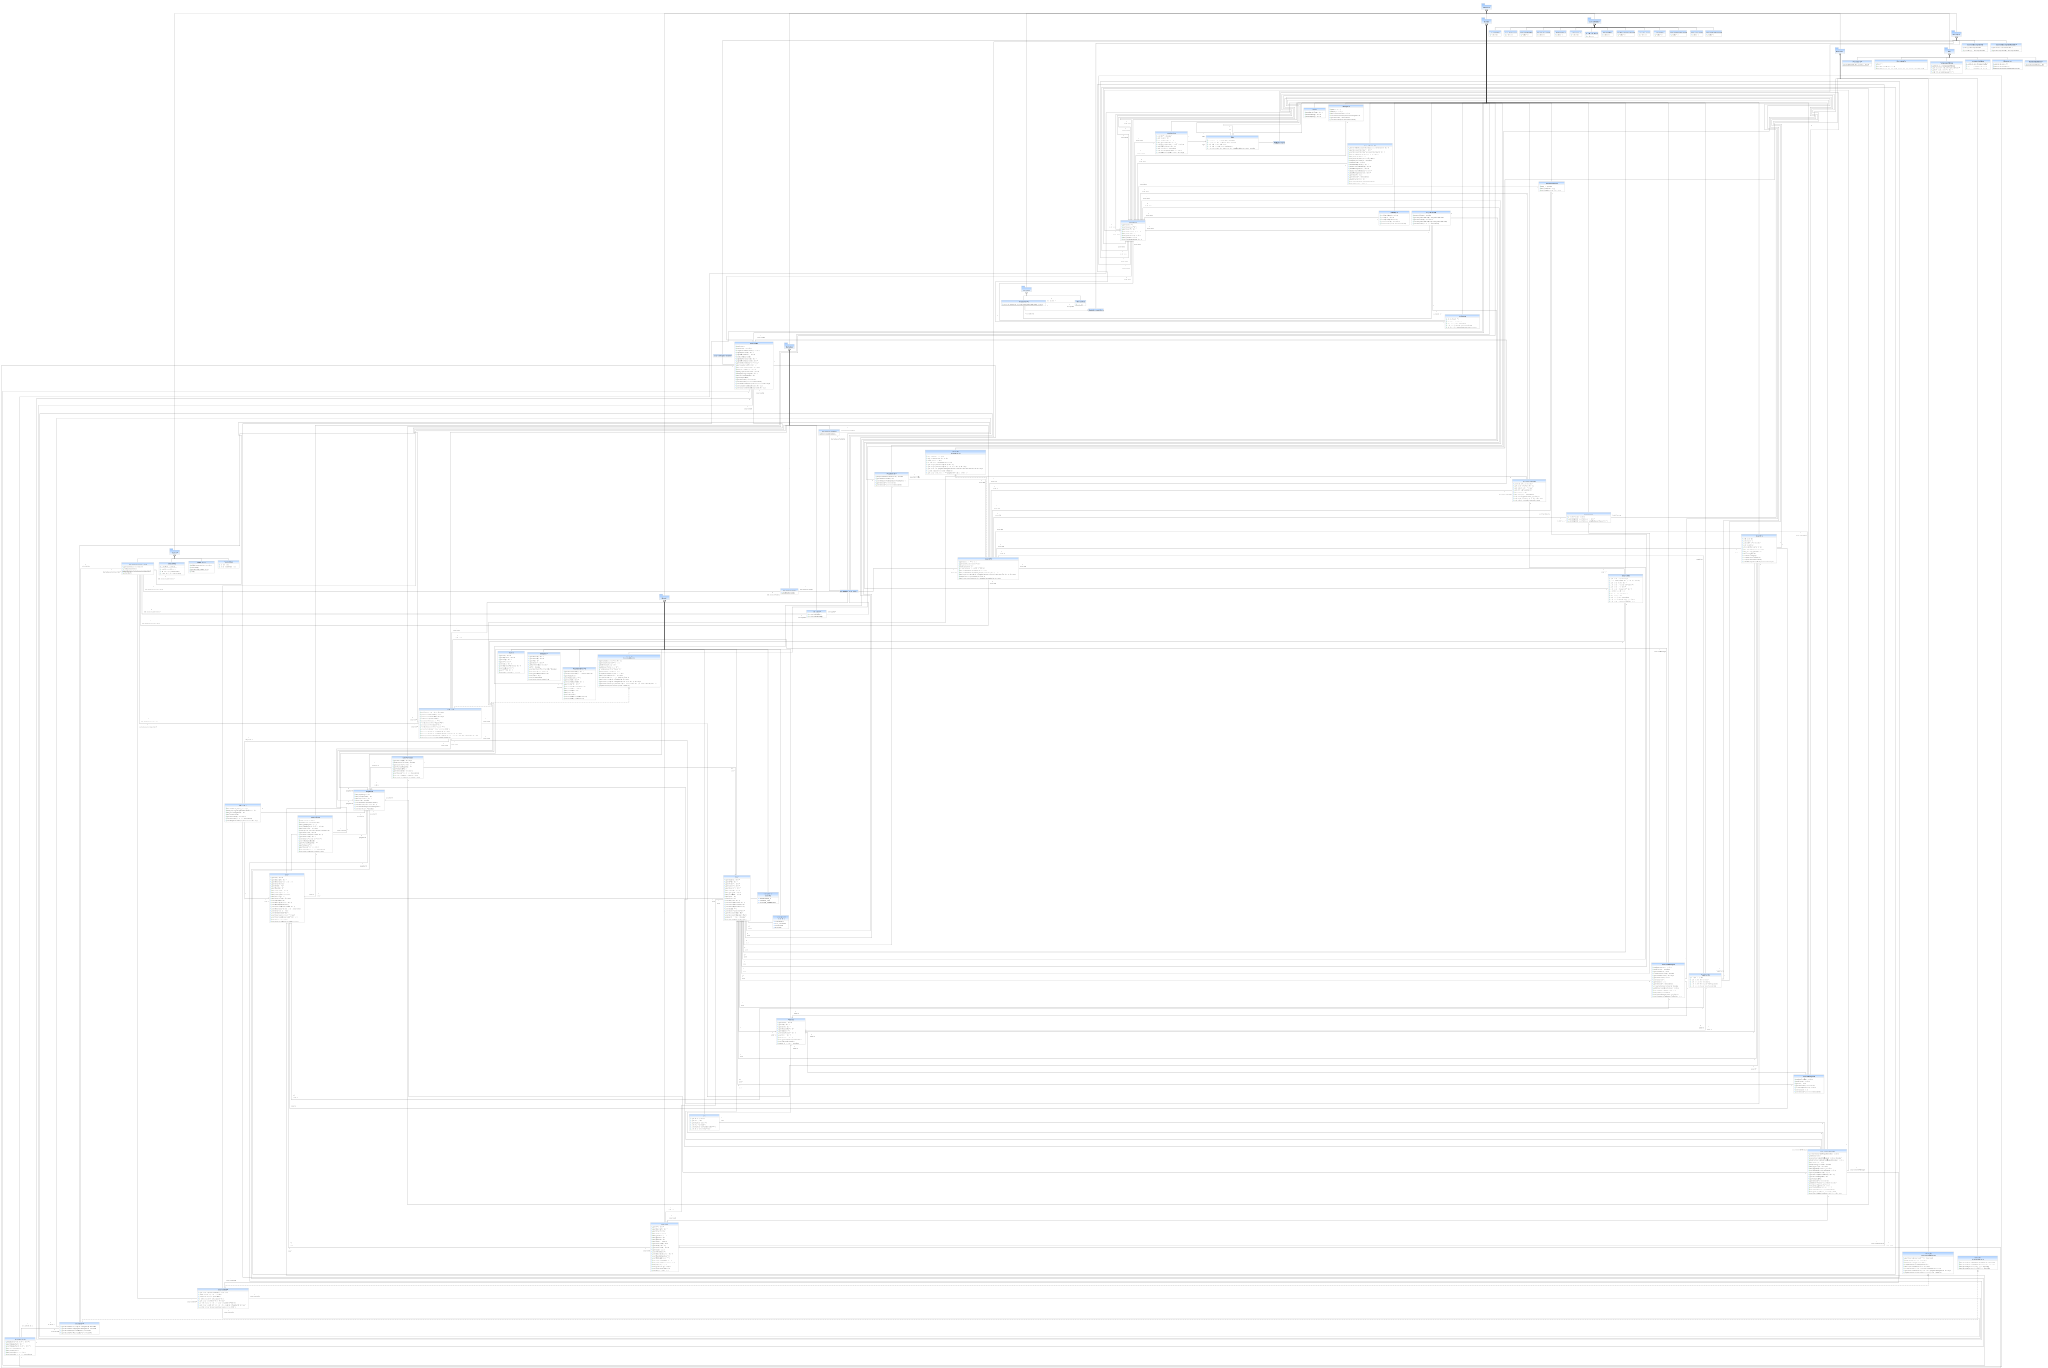
\includegraphics[width=0.9\linewidth]{Grafiken/UMLKlassendiagramm}
			\caption{UML-Klassendiagramm des ofCourse-Systems}
		\end{figure}
	


